\date{}
\title{}
\date{}
\begin{document}
\begin{frame}
    \titlepage
\end{frame}


\makeatletter
\newenvironment<>{btHighlight}[1][]
{\begin{onlyenv}#2\begingroup\tikzset{bt@Highlight@par/.style={#1}}\begin{lrbox}{\@tempboxa}}
{\end{lrbox}\bt@HL@box[bt@Highlight@par]{\@tempboxa}\endgroup\end{onlyenv}}

\newcommand<>\btHL[1][]{%
  \only#2{\begin{btHighlight}[#1]\bgroup\aftergroup\bt@HL@endenv}%
}
\def\bt@HL@endenv{%
  \end{btHighlight}%   
  \egroup %
}
\tikzset{
    btHLbox/.style={
        fill=red!30,outer sep=0pt,inner xsep=1pt, inner ysep=0pt, rounded corners=3pt
    },
}
\newcommand{\bt@HL@box}[2][]{%
  \tikz[#1]{%
    \pgfpathrectangle{\pgfpoint{1pt}{0pt}}{\pgfpoint{\wd #2}{\ht #2}}%
    \pgfusepath{use as bounding box}%
    \node[text width={},draw=none,anchor=base west, btHLbox, minimum height=\ht\strutbox+1pt,#1]{\raisebox{1pt}{\strut}\strut\usebox{#2}};
  }%
}

\lst@CCPutMacro
    \lst@ProcessOther {"2A}{%
      \lst@ttfamily 
         {\raisebox{2pt}{*}}% used with ttfamily
         {\raisebox{2pt}{*}}}% used with other fonts
    \@empty\z@\@empty

\lstdefinelanguage
   [x8664gas]{Assembler}     % add a "x64" dialect of Assembler
   [x86masm]{Assembler} % based on the "x86masm" dialect
   % with these extra keywords:
   {morekeywords={CDQE,CQO,CMPSQ,CMPXCHG16B,JRCXZ,LODSQ,MOVSXD,%
                  POPFQ,PUSHFQ,SCASQ,STOSQ,IRETQ,RDTSCP,SWAPGS,.TEXT,.STRING,.ASCIZ,%
                  BEQ,LW,SW,LB,SB,ADDIU,J,BEQZ,BNEZ,BNE,%
                  MOVUPD,MULPD,MOVSD,MULSD,%
                  SHLADD,MOV,CMP.LT,TBIT.NZ,BR.RET.SPTK.MANY,%
                  ADDQ,POPQ,PUSHQ,RRMOVQ,MRMOVQ,RMMOVQ,IRMOVQ,%
                  <-,LL,SC,ADDI,ADDL,VMOVDQA,ADDQ,CMPL,JB,JBE,MOVL,CLTQ,
                  MOVW,PUSHW,MOV,ADD,SUB,INT,PUSH,MOV,ADD,REP,MOVSB,%
                  TESTQ,CMPQ,MOVL,MOVQ,ADDQ,JMPQ,XORQ,%
                  LEAQ,LEAL,LEA,RETQ,RET,POPL,POPW,PUSHL,PUSHW,%
                  LEAW,%
                  SUBQ,SYSCALL,.ASCII,CALLQ,MOVSLQ,JMP,ANDQ,SHRQ,MOVB,INCQ,TESTL,XORL,%
                  SHRL,LEAL,SARL,SUBL,IMULL,IMULQ,MOVDQU,PADDD,XORL,%
                  MOVZBL,MOVZB,SHRB,SRAL,SHRL,ANDL,%
                  CMOVNS,SRAL,SRAQ,MOVZBW,MOVZBQ,%
                  PADDW,PADDQ,MODUPS,MOVAPD,%
                  MOVL,RET,.GLOBL,%
                  },
    deletekeywords={eax,ebx,sp,si,cx,di,ds,cs,es,fs,dx,ax,bx,al,esi,ebp,ecx,rip,eip,edx,edi,rdi,esp},
    morecomment=[l]{\#},
    morecomment=[l]{\/\/},
    morecomment=[s]{/*}{*/},
    sensitive=false,
    keepspaces=true} % et

\lstalias[]{myasm}[x8664gas]{Assembler}

\lstdefinelanguage{JavaScript}{
  keywords={typeof, new, true, false, catch, function, return, null, catch, switch, var, if, in, while, do, else, case, break},
  ndkeywords={class, export, boolean, throw, implements, import, this},
  sensitive=false,
  comment=[l]{//},
  morecomment=[s]{/*}{*/},
  morestring=[b]',
  morestring=[b]"
}

\newcommand{\keywordstyle}{\sourcecodeprolight\bfseries\color{blue!30!black}}
\newcommand{\stringstyle}{\color{blue!20!black}\ttfamily}

\lstset{
    language=C,
    basicstyle=\sourcecodepro\EmptyMapping,
    escapechar=`,
    keywordstyle=\keywordstyle\EmptyMapping,
    identifierstyle=\sourcecodepro\EmptyMapping,
    numberstyle=\small\color{black!70},
    commentstyle=\color{red!60!black}\ttfamily\itshape,
    stringstyle=\color{blue!20!black}\ttfamily,
    ndkeywordstyle=\bfseries\color{blue!30!black},
    upquote=true,
}



\lstdefinestyle{medium}{
    basicstyle=\sourcecodepro\EmptyMapping\fontsize{12}{13}\selectfont,
    keywordstyle=\sourcecodepro\EmptyMapping\fontsize{12}{13}\selectfont\keywordstyle,
}

\lstdefinestyle{small}{
    basicstyle=\sourcecodepro\EmptyMapping\small,
    keywordstyle=\sourcecodepro\EmptyMapping\small\keywordstyle,
}

\lstdefinestyle{smaller}{
    basicstyle=\sourcecodepro\EmptyMapping\fontsize{11}{12}\selectfont,
    keywordstyle=\sourcecodepro\EmptyMapping\fontsize{11}{12}\selectfont\keywordstyle,
}


\lstdefinestyle{script}{
    basicstyle=\sourcecodepro\EmptyMapping\scriptsize,
    keywordstyle=\sourcecodepro\EmptyMapping\scriptsize\bfseries,
}




\section{some malicious things we'd like to stop}

\begin{frame}<1>[label=portalShouldnt]\frametitle{things programs on portal shouldn't do}
    \begin{itemize}
    \item \myemph<2>{read other user's files}
    \item \myemph<3>{modify OS's memory}
    \item \myemph<3>{read other user's data in memory}
    \item \myemph<4>{hang the entire system}
    \end{itemize}
\end{frame}


\section{privileged instruction idea}
\againframe<2>{portalShouldnt}
\begin{frame}{privileged instructions}
\begin{itemize}
\item can't let \myemph{any program} run some instructions
\item example: talk to I/O device
\item allows machines to be shared between users (e.g. lab servers)
\vspace{.5cm}
\item processor has two modes:
\begin{itemize}
    \item kernel mode --- privileged instructions work
    \item user mode --- privileged instructions cause exception instead
\end{itemize}
\item only \textit{trusted} OS code runs in kernel mode
\end{itemize}
\end{frame}

\begin{frame}{kernel mode}
\begin{itemize}
\item extra one-bit register: ``are we in kernel mode''
\vspace{.5cm}
\item processor switches to kernel mode to run OS
\item OS switches processor back to use mode when running normal code
\end{itemize}
\end{frame}




\section{system calls: running the OS}
\usetikzlibrary{arrows.meta,decorations.pathreplacing,patterns}


\ifdefined\codeBoxA\else\newsavebox\codeBoxA\fi
\begin{lrbox}{\codeBoxA}
\lstset{language=C++}
\begin{lstlisting}
void readFromDiskInto(int diskLocation, char *dest) {
    ...
    runPrivilegedInstruction(...);
    ...
}
\end{lstlisting}
\end{lrbox}
\ifdefined\codeBoxB\else\newsavebox\codeBoxB\fi
\begin{lrbox}{\codeBoxB}
\lstset{language=C++}
\begin{lstlisting}
void readFileSafely(const char *name, char *dest) {
    if (canCurrentProgramCanAccessFile(name)) {
        readFromDiskInto(lookupFile(name), dest)
    }
}
\end{lstlisting}
\end{lrbox}

\begin{frame}[fragile,label=callOSDirectP]{calling the OS?}
\begin{tikzpicture}
\draw[fill=blue!10] (0, 0) rectangle ++(2, -3);
\draw[fill=green!10] (0, -3) rectangle ++(2, -3);
\draw[thick] (0, 0) rectangle ++(2, -6);
\draw[very thick,decorate,decoration={brace,mirror}] (-.25, 0) -- ++(0, -3)
    node[midway,left] {OS code};
\draw[very thick,decorate,decoration={brace,mirror}] (-.25, -3) -- ++(0, -3)
    node[midway,left] {program code};
% FIXME: pointer to functions in OS
\draw[thin,pattern=north west lines] (0.5, -1) rectangle ++(1.0, -.2);
\draw[thin,pattern=vertical lines] (0.8, -2) rectangle ++(1.0, -.1);
\draw (1.5, -1.0) -- ++(1cm, 1cm) node[draw,very thick,anchor=north west,font=\tt\scriptsize] (readFromDiskInto) {
\usebox{\codeBoxA}
};
\draw (1.5, -1.2) -- (readFromDiskInto.south west);

\draw (1.8, -2.0) -- ++(.8cm, -.25cm) node[draw,very thick,anchor=north west,font=\tt\scriptsize] (readFileSafely) {
\usebox{\codeBoxB}
};
\draw (1.8, -2.1) -- (readFileSafely.south west);

\draw[very thick,Latex-] (1.2, -5) -- ++ (2cm, -.25cm) node[right,align=left] {
    how do we let this code run \\
    \texttt{readFileSafely} in kernel mode \\
    but not \texttt{readFromDisk}?
};
% FIXME: pointer to user code
\end{tikzpicture}
\end{frame}
 % FIXME: incomplete
    % special switch to OS function
    % can't let us just call an OS function directly

\subsection{exception entry point}


\begin{frame}{controlled entry to kernel mode (1)}
\begin{itemize}
\item special instruction: ``system call''
\vspace{.5cm}
\item runs OS code in kernel mode at location specified earlier 
\item OS sets up at boot
\item location can't be changed without privilieged instrution
\end{itemize}
\end{frame}

\begin{frame}{controlled entry to kernel mode (2)}
\begin{itemize}
\item OS needs to make specified location:
\vspace{.5cm}
\item figure out what operation the program wants
    \begin{itemize}
    \item calling convention, similar to function arguments + return value
    \end{itemize}
\item be ``safe'' --- not allow the program to do `bad' things
    \begin{itemize}
    \item example: checks whether current program is allowed to read file before reading it
    \item requires exceptional care --- program can try weird things
    \end{itemize}
\end{itemize}
\end{frame}


\subsection{system calls on Linux}
% FIXME import slides
\begin{frame}{Linux x86-64 system calls}
\begin{itemize}
\item special instruction: {\tt syscall}
\item runs OS specified code in kernel mode
\end{itemize}
\end{frame}

\begin{frame}[fragile,label=LinuxSyscall]{Linux syscall calling convention}
\begin{itemize}
\item before {\tt syscall}:
\item \lstinline|%rax| --- system call number
\item \lstinline|%rdi|, \lstinline|%rsi|, \lstinline|%rdx|, \lstinline|%r10|, \lstinline|%r8|, \lstinline|%r9| --- args
\vspace{.5cm}
\item after {\tt syscall}:
\item \lstinline|%rax| --- return value
\item on error: \lstinline|%rax| contains -1 times ``error number''
\vspace{.5cm}
\item \myemph{almost} the same as normal function calls
\end{itemize}
\end{frame}

\begin{frame}{Linux x86-64 hello world}
\lstset{language=myasm,style=small,morekeywords={syscall,movq,.asciz,.globl}}
\lstinputlisting{../kernel/hello_world.s}
\end{frame}

\begin{frame}[fragile,label=sysHandler]{approx. system call handler}
\lstset{
    language=myasm,
    morekeywords={.quad,pushq,jmp},
    escapechar=@,
    style=small,
}
\begin{lstlisting}
sys_call_table:
    .quad handle_read_syscall
    .quad handle_write_syscall
    // ...

handle_syscall:
    ... // save old PC, etc.
    pushq %rcx // save registers
    pushq %rdi
    ...
    call *sys_call_table(,%rax,8)
    ...
    popq %rdi
    popq %rcx
    return_from_exception
\end{lstlisting}
\end{frame}

% FIXME: kernel stack diagram

\begin{frame}{Linux system call examples}
\begin{itemize}
\item {\tt mmap}, {\tt brk} --- allocate memory
\item {\tt fork} --- create new process
\item {\tt execve} --- run a program in the current process
\item {\tt \myemph<2>{\_exit}} --- terminate a process
\item {\tt open}, {\tt \myemph<2>{read}}, {\tt write} --- access files
\item {\tt socket}, {\tt accept}, {\tt getpeername} --- socket-related
\end{itemize}
\end{frame}



\subsection{system call wrappers}
\begin{frame}{system call wrappers}
    \begin{itemize}
    \item can't write C code to generate syscall instruction
    \item solution: call ``wrapper'' function written in assembly
    \end{itemize}
\end{frame}


\section{kernel + standard library}

% FIXME: diagram of kernel + standard library from whatisos
\usetikzlibrary{matrix,decorations.pathreplacing}

\begin{frame}<1-5>[fragile,label=classicUnix]{the classic Unix design}
\begin{tikzpicture}
\tikzset{
    user/.style={fill=blue!10},
    iface/.style={fill=black!15},
    kernel/.style={fill=red!10},
    hardware/.style={},
}
% FIXME: show standard libraries/etc. can use HW directly
\matrix[tight matrix,
        nodes={draw,thick,text width=13cm,align=left},
        ] {
    |[minimum height=1cm,alias=apps,user]| applications \\
    |[minimum height=0.5cm,alias=slibiface,iface,text width=11cm,xshift=1cm]| standard library functions / shell commands \\
    |[minimum height=1cm,alias=stdlib,user,text width=11cm,xshift=1cm]| {standard libraries and \\utility programs} \\
    |[minimum height=0.5cm,alias=syscalls,iface,text width=9.5cm,xshift=1.75cm]| system call interface \\
    |[minimum height=2cm,alias=kernel,kernel,text width=9.5cm,xshift=1.75cm]| kernel \\
    |[minimum height=1cm,alias=hwIface,iface]| \hspace{2cm}\only<1>{hardware interface}~ \\
    |[minimum height=1.5cm,alias=hw,hardware]| hardware \\
};
\path[iface] (hwIface.north west) -- ++(3.5cm, 0cm) |- (stdlib.south west) |- (apps.south west) -- cycle;
\path[draw,very thick,black!15] ([xshift=3.5cm]hwIface.north west) -- (hwIface.north west);
\path[draw,thick] ([xshift=3.5cm]hwIface.north west) |- (stdlib.south west) |- (apps.south west) -- (hwIface.north west);
\begin{visibleenv}<2->
\path[draw,very thick,dotted] (kernel.south west) -- ++(0cm, -1cm);
\node[align=center,alt=<3>{red},alt=<6>{red}] at ([xshift=1.5cm,yshift=1cm]hwIface.north west) {
    user-mode \\
    hardware \\
    interface \\
    (limited)
};
\node[anchor=north,alt=<2>{red},alt=<6>{red}] at (kernel.south) {
    kernel-mode hardware interface (complete)
};
\end{visibleenv}
\tikzset{
    component parts/.style={font=\small,anchor=east,align=left}
}
\node[text width=8cm,minimum height=2cm,component parts] at (kernel.east) {
    \begin{tabular}{lll}
    CPU scheduler & filesystems & networking \\
    virtual memory & device drivers & signals \\
    pipes & swapping & \ldots
    \end{tabular}
};
\node[text width=6cm,minimum height=1cm,component parts] at (stdlib.east) {
    \begin{tabular}{ll}
    libc (C standard library) & the shell\\
    login & login\ldots \\
    \end{tabular}
};
\node[text width=10cm,minimum height=1cm,component parts] at (hw.east) {
    \begin{tabular}{lll}
    memory management unit & device controllers & \ldots \\
    \end{tabular}
};
\begin{visibleenv}<4>
\draw[ultra thick,decorate,decoration={brace}] ([xshift=.25cm]slibiface.north east) -- ([xshift=.25cm]kernel.south east) 
    node[midway,right] {the OS?};
\end{visibleenv}
\begin{visibleenv}<5>
\draw[ultra thick,decorate,decoration={brace}] ([xshift=.5cm]syscalls.north east) -- ([xshift=.5cm]kernel.south east) 
    node[midway,right] {the OS?};
\end{visibleenv}
\end{tikzpicture}
\end{frame}

\begin{frame}{aside: is the OS the kernel?}
    \begin{itemize}
    \item OS = stuff that runs in kernel mode?
    \item OS = stuff that runs in kernel mode + libraries to use it?
    \item OS = stuff that runs in kernel mode + libraries + utility programs (e.g. shell, finder)?
    \item OS = everything that comes with machine?
    \vspace{.5cm}
    \item no consensus on where the line is
    \item each piece can be replaced separately\ldots
    \end{itemize}
\end{frame}



\section{memory protection}
\againframe<3>{portalShouldnt}

\subsubsection{exercise: expected behavior?}
\usetikzlibrary{positioning,shapes.multipart}

\begin{frame}<1-2>[label=memProtectQ]{memory protection}
\begin{itemize}
    \item modifying another program's memory?
\end{itemize}
\lstset{language=myasm,style=small,morekeywords={movq,.word}}
\begin{tabular}{l@{\hspace{.5cm}}|@{\hspace{.5cm}}l}
Program A & Program B \\ \hline
\lstinputlisting{../kernel/memprot-ex1.c} & \lstinputlisting{../kernel/memprot-ex2.c} \\ \hline
~ & ~ \\
\only<2>{result: {\tt \%rax} (in A) is \ldots} 
\only<3->{result: {\tt \%rax} (in A) is {\tt 42} (always)} &
\only<4>{result: {\tt \%rax} (in B) is \ldots} 
\only<5->{result: \myemph{might crash}} \\
\end{tabular}

\begin{visibleenv}<2-5>
\small
A. 42 \hspace{1cm} B. 99 \hspace{1cm} C. 0x10000  \\
D. 42 or 99 (depending on timing/program layout/etc) \\
E. 42 or 99 or program might crash (depending on \ldots) \\
F. something else \\
\end{visibleenv}
\end{frame}

\iftoggle{heldback}{}{\againframe<3>{memProtectQ}}


\subsubsection{address spaces}
\usetikzlibrary{arrows.meta,calc,fit,positioning,patterns,shapes.multipart}

\begin{frame}<1>[label=progMem]{program memory (two programs)}
\begin{tikzpicture}
\tikzset{
    mylabel/.style={font=\ttfamily},
    mybox/.style={draw,rectangle,minimum width=5cm,fill=white,inner sep=1mm},
    myhigh/.style={draw,rectangle,line width=1mm, draw=blue!80!black,opacity=.3},
}
\begin{scope}[name prefix=A-]
\node[mybox,minimum height=1cm,pattern=north west lines,pattern color=black!5!white] (kernel) {Used by OS};
\node[above=0cm of kernel] {Program A};
\node[mybox, minimum height=.5cm, below=1cm of kernel] (stack) {Stack};
\node[mybox, minimum height=.5cm, below=1cm of stack] (heap) {Heap / other dynamic};
\node[mybox, minimum height=.5cm, below=0mm of heap] (data) {Writable data};
\node[mybox, minimum height=.5cm, below=0mm of data] (sdata) {Code + Constants};
\coordinate (memBottom) at ($(sdata.south east) + (0mm, -2mm)$);
\begin{pgfonlayer}{bg}
\draw[pattern=north west lines, pattern color=black!40!white] (kernel.north west) rectangle (memBottom);
\end{pgfonlayer}
\end{scope}

\begin{scope}[name prefix=B-,xshift=6cm]
\node[mybox,minimum height=1cm,pattern=north west lines,pattern color=black!5!white] (kernel) {Used by OS};
\node[above=0cm of kernel] {Program B};
\node[mybox, minimum height=.6cm, below=1cm of kernel] (stack) {Stack};
\node[mybox, minimum height=1.4cm, below=.3cm of stack] (heap) {Heap / other dynamic};
\node[mybox, minimum height=.5cm, below=0mm of heap] (data) {Writable data};
\node[mybox, minimum height=.5cm, below=0mm of data] (sdata) {Code + Constants};
\coordinate (memBottom) at ($(sdata.south east) + (0mm, -2mm)$);
\begin{pgfonlayer}{bg}
\draw[pattern=north west lines, pattern color=black!40!white] (kernel.north west) rectangle (memBottom);
\end{pgfonlayer}
\end{scope}

\begin{visibleenv}<2>
\node[myhigh,fit=(A-heap.north west) (A-stack.south east)] {};
\node[myhigh,fit=(B-heap.north west) (B-stack.south east)] {};
\node[myhigh,fit=(A-memBottom) (A-sdata.south west)] {};
\node[myhigh,fit=(B-memBottom) (B-sdata.south west)] {};
\node[myhigh,fit=(A-stack.north west) (A-kernel.south east)] {};
\node[myhigh,fit=(B-stack.north west) (B-kernel.south east)] {};
\end{visibleenv}

\begin{visibleenv}<3>
\node[myhigh,fit=(A-kernel)] {};
\node[myhigh,fit=(B-kernel)] {};
\end{visibleenv}
\end{tikzpicture}
\end{frame}

\begin{frame}<1>[label=addrSpace]{address space}
\begin{itemize}
\item programs have \myemph{illusion of own memory}
\item called a program's \myemph{address space}
\end{itemize}
\begin{tikzpicture}
\tikzset{
    every node/.style={font=\small},
}
\node[align=center] (progAAddr) {Program A \\ addresses};
\node[below=1cm of progAAddr,align=center] (progBAddr) {Program B \\ addresses};
\node[draw, right=1cm of progAAddr,align=center] (translationA) { mapping \\ (set by OS) };
\node[draw, right=1cm of progBAddr,align=center] (translationB) { mapping \\ (set by OS) };
\node[draw,rectangle split, rectangle split parts=6, anchor=north west,label={north:real memory}] (mem) at ([xshift=1cm]translationA.north east) {
    \nodepart{one}
    Program A code 
    \nodepart{two}
    Program B code
    \nodepart{three}
    Program A data
    \nodepart{four}
    Program B data
    \nodepart{five}
    OS data
    \nodepart{six}
    \ldots
};
\draw[-Latex,green,thick] (progAAddr) -- (translationA) (translationA.east) -- (mem.one west);
\draw[-Latex,green,thick] (translationA.east) -- (mem.three west);
\draw[-Latex,blue,thick] (progBAddr) -- (translationB) (translationB.east) -- (mem.two west);
\draw[-Latex,blue,thick] (translationB.east) -- (mem.four west);
\begin{visibleenv}<2->
    \node[thick,red,draw,anchor=north west] (error) at ([yshift=-.5cm]mem.south west) {trigger error};
    \draw[-Latex,green,thick] (translationA.east) -- (error.west);
    \draw[-Latex,blue,thick] (translationB.east) -- (error.west);
\end{visibleenv}
\begin{visibleenv}<3>
    \draw[-Latex,green,ultra thick,dotted] (translationA.east) -- (mem.five west);
    \draw[-Latex,blue,ultra thick,dotted] (translationB.east) -- (mem.five west);
    \draw[-Latex,ultra thick,dotted] ([xshift=-3cm,yshift=-.5cm]translationB.south) -- ([xshift=-2cm,yshift=-.5cm]translationB.south)
        node[right] {= kernel-mode only};
\end{visibleenv}
\end{tikzpicture}
\end{frame}

\againframe<2>{progMem}

\againframe<2>{addrSpace}

\begin{frame}{address space mechanisms}
\begin{itemize}
\item topic after exceptions
\item called \myemph{virtual memory}
\item mapping called \myemph{page tables}
\item mapping part of what is changed in context switch
\end{itemize}
\end{frame}




\section{infinite loop}
\againframe<4>{portalShouldnt}

\begin{frame}{an infinite loop}
\lstinputlisting[language=C]{../kernel/loop.c}
\begin{itemize}
\item If I run this on a shared department machine, can you still use it? \\
\ldots if the machine only has one core?
\end{itemize}
\end{frame}

\begin{frame}{timing nothing}
\lstinputlisting[firstline=18,language=C]{../kernel/timedloop.c}
\begin{itemize}
\item same instructions --- \myemph{same difference} each time?
\end{itemize}
\end{frame}

\begin{frame}{doing nothing on a busy system}
    % FIXME: wider versions?
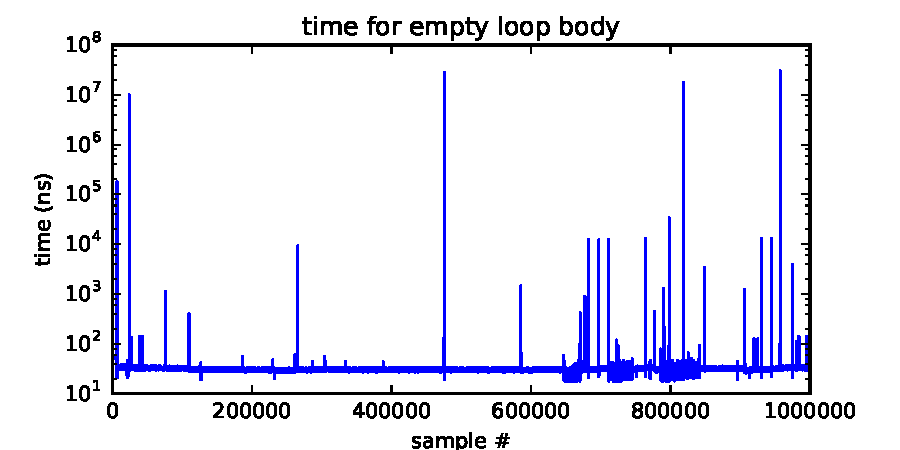
\includegraphics[width=\textwidth]{../kernel/empty-samples}
\end{frame}

\begin{frame}{doing nothing on a busy system}
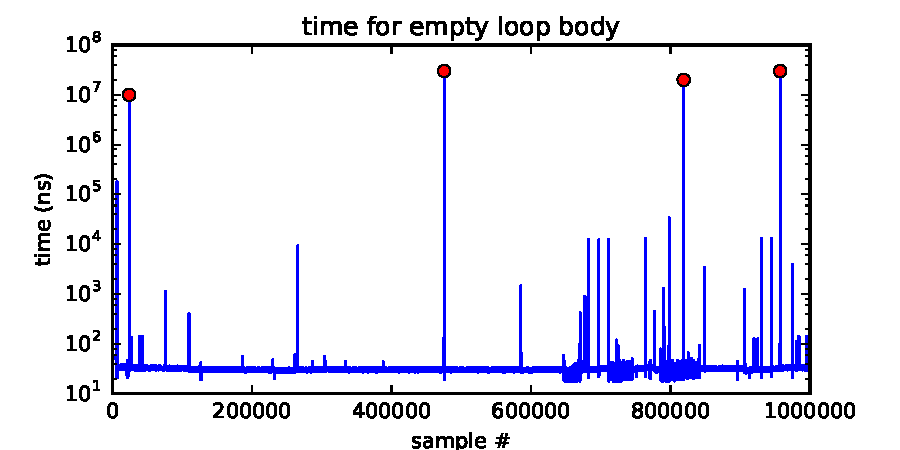
\includegraphics[width=\textwidth]{../kernel/empty-samples-big-marked}
\end{frame}



\usetikzlibrary{arrows.meta}

\begin{frame}[fragile,label=timeMulti1]{time multiplexing}
\begin{tikzpicture}
\tikzset{
    prog1/.style={draw,fill=cyan!70},
    prog2/.style={draw,fill=green,visible on=<3->},
    prog3/.style={draw,fill=violet!30,visible on=<3->},
    proglabel/.style={font=\tt\scriptsize},
    labelprog1/.style={execute at begin node={\strut loop.exe}},
    labelprog2/.style={execute at begin node={\strut ssh.exe},visible on=<3->},
    labelprog3/.style={execute at begin node={\strut firefox.exe},visible on=<3->},
}

\begin{scope}[xscale=1.5,yscale=1]
\foreach \s/\e/\p [count=\x] in {0/2/1,2/3/2,3/5/3,5/6/1,6/7/2}{
    \draw[prog\p] (\s, 0) rectangle (\e, 1) coordinate[midway] (mid-\x);
    \node[anchor=center,proglabel,labelprog\p] at (mid-\x) {};
}
\end{scope}
\node[anchor=east] at (-0.25, 0.5) {CPU:};
% FIXME: system
\begin{scope}[yscale=1,yshift=-2.5mm]
\draw[thick,-Latex] (1,0) node[left] {time} -- (10.5,0);
\end{scope}
\begin{visibleenv}<2->
    \begin{scope}[xscale=1.5]
    \draw[red,thick] (1.9,-.1) coordinate (firstStart) rectangle (2.0, 1.1);
    \draw[red,thick] (5.1,-.1) coordinate (lastEnd) rectangle (5.0, 1.1);
    \end{scope}
    \node[anchor=north west] (asmPre) at (0, -1) {
\begin{lstlisting}[language=myasm,style=small]
...
call get_time 
    // whatever get_time does
movq %rax, %rbp
\end{lstlisting}
    };
    \draw[red, ultra thick] ([yshift=-.2cm]asmPre.south west) -- ([yshift=-.2cm]asmPre.south east) node [draw=none,midway,fill=white,
        inner sep=3pt] 
        {million cycle delay};
    \node[anchor=north west] (asmPost) at ([yshift=-.5cm]asmPre.south west) {
\begin{lstlisting}[language=myasm,style=small]
call get_time
    // whatever get_time does
subq %rbp, %rax
...
\end{lstlisting}
    };
\end{visibleenv}
\end{tikzpicture}
\end{frame}




\section{reasons for exceptions, generally}

\usetikzlibrary{decorations.pathreplacing}

\begin{frame}<0>[label=exceptTypesN]{types of exceptions}
\begin{itemize}
\item \tikzmark{int bot}\myemph<3>{externally-triggered}
    \begin{itemize}
    \item \myemph<3>{timer} --- keep program from hogging CPU
    \item \myemph<4>{I/O devices} --- key presses, hard drives, networks, \ldots
    \item \tikzmark{abort bot}hardware is broken (e.g. memory parity error)
    \end{itemize}
\item \tikzmark{trap bot}intentionally triggered exceptions
    \begin{itemize}
    \item \myemph<5>{system calls} --- ask OS to do something
    \end{itemize}
\item \tikzmark{fault bot}\myemph<6>{errors/events in programs}
    \begin{itemize}
        \item \myemph<7>{memory not in address space} (``Segmentation fault'')
        \item \myemph<8>{privileged instruction}
    \item divide by zero
    \item invalid instruction\tikzmark{invalid}
    \end{itemize}
\end{itemize}
\begin{tikzpicture}[overlay,remember picture]
    \coordinate (int top) at ([yshift=.6cm]pic cs:int bot);
    \coordinate (fault top) at ([yshift=.6cm]pic cs:fault bot);
    \coordinate (trap top) at ([yshift=.6cm]pic cs:trap bot);
    \coordinate (fault bot) at (pic cs:fault bot);
    \coordinate (over) at ([xshift=-4.5cm]current page.east);
    \coordinate (abort bot)  at (pic cs:abort bot);
    \coordinate (invalid bot)  at ([yshift=.6cm]pic cs:invalid bot);
    \draw[very thick,decorate,decoration={brace}] (int top -| over) -- (abort bot -| over) 
        node[midway,right,font=\large] (async label) {\myemph<2>{asynchronous}};
        \node[anchor=north west,font=\small,align=left] at ([xshift=.15cm,yshift=.3cm]async label.south west) {
            not triggered by \\
            running program
        };
    \draw[very thick,decorate,decoration={brace}] (trap top -| over) -- (invalid bot -| over) 
        node[midway,right,font=\large] (sync label) {\myemph<2>{synchronous}};
        \node[anchor=north west,font=\small,align=left] at ([xshift=.15cm,yshift=.3cm]sync label.south west) {
            triggered by \\
            current program
        };
\end{tikzpicture}
\end{frame}

\againframe<1>{exceptTypesN}


\subsection{aside: terms}
\begin{frame}{terms for exceptions}
    \begin{itemize}
    \item terms for exceptions aren't standardized
    \vspace{.5cm}
    \item our readings use one set of terms
    \begin{itemize}
        \item interrupts = externally-triggered
        \item faults = error/event in program
        \item trap = intentionally triggered
        \end{itemize}
    \item all these terms appear differently elsewhere
    \end{itemize}
\end{frame}


\section{exception table + dispatch}

\begin{frame}{exception implementation}
\begin{itemize}
\item detect condition (program error or external event)
\item save current value of PC somewhere
\item jump to \myemph{exception handler} (part of OS)
    \begin{itemize}
    \item jump done without program instruction to do so
    \end{itemize}
\end{itemize}
\end{frame}

\begin{frame}{exception implementation: notes}
\begin{itemize}
\item I describe a \myemph{simplified} version
\item real x86/x86-64 is a bit more complicated
    \begin{itemize}
    \item (mostly for historical reasons)
    \end{itemize}
\end{itemize}
\end{frame}

\begin{frame}[label=locating,fragile]{locating exception handlers}
\begin{tikzpicture}
\tikzset{
    >=Latex,
    every node/.style={font=\small},
}
\matrix[tight matrix,
    nodes={text width=2.5cm,font=\small},
    column 1/.append style={nodes={draw=none}},
    column 2/.append style={nodes={text width=1.5cm}},
    row 1/.append style={nodes={draw=none}},
    label={[inner sep=0mm,align=center]north:{{\bfseries exception table} (in memory)}},
    label distance=1mm,
] (eTable) {
    |[align=center]| address \& pointer \\
    base + {\tt 0x00} \& ~ \\
    base + {\tt 0x08} \& ~ \\
    base + {\tt 0x10} \& ~ \\
    base + {\tt 0x18} \& ~ \\
    |[align=center]| \ldots \& |[draw=none,align=center]| \ldots \\
    base + {\tt 0x40} \&  ~ \\
    |[align=center]| \ldots \& |[draw=none,align=center]| \ldots \\
};
\node[draw,text width=2.8cm, align=center, anchor=south] (baseReg) at ([yshift=1cm,xshift=5mm]eTable-1-1.north west){ exception table base register };
\draw[dashed,very thick,->] ([xshift=-1.2cm]baseReg.south) |- (eTable-2-1.west);
\node[draw,anchor=north west] (hDivZero) at ([xshift=2cm,yshift=2cm]eTable-2-2.north east) {
\begin{lstlisting}[style=script,language=myasm]
handle_divide_by_zero:
  movq %rax, save_rax
  movq %rbx, save_rbx
  ...
\end{lstlisting}
};
\node[draw,anchor=north west] (hTimer) at ([yshift=-2.5cm]hDivZero.south west){
\begin{lstlisting}[style=script,language=myasm]
handle_timer_interrupt:
  movq %rax, save_rax
  movq %rbx, save_rbx
  ...
\end{lstlisting}
};
\draw[->,thick] (eTable-2-2.center) -- ++(2,0) |- ([yshift=-1ex]hDivZero.north west);
\draw[thick] (eTable-3-2.center) -- ++ (2, 0) node[right]{\ldots};
\draw[thick] (eTable-4-2.center) -- ++ (2, 0) node[right]{\ldots};
\draw[thick] (eTable-5-2.center) -- ++ (2, 0) node[right]{\ldots};
\draw[->,thick] (eTable-7-2.center) -- ++(2,0) |- ([yshift=-1ex]hTimer.north west);
\end{tikzpicture}
\end{frame}

\begin{frame}[fragile,label=exceptHandlerRun]{running the exception handler}
\begin{itemize}
    \item hardware saves the \myemph{old program counter} (and maybe more)
    \item identifies location of exception handler via table
    \item then jumps to that location
    \vspace{.5cm}
    \item OS code can save anything else it wants to , etc.
\end{itemize}
\end{frame}




\section{context switches} % FIXME: move earlier???
    % FIXME: simplify diagram
    % FIXME: include address space as part of context
\usetikzlibrary{arrows.meta,calc,positioning,matrix,patterns}

\begin{frame}{switching programs}
% FIXME: picture showing zoom of timeline
\begin{itemize}
\item OS starts running somehow
    \begin{itemize}
    \item some sort of exception
    \end{itemize}
\item saves old registers + program counter + address mapping
    \begin{itemize}
    \item (optimization: could omit when program crashing/exiting)
    \end{itemize}
\item sets new registers + address mapping, jumps to new program counter
\item called \myemph{context switch}
    \begin{itemize}
    \item saved information called \myemph{context}
    \end{itemize}
\end{itemize}
\end{frame}

\tikzset{a/.style={fill=blue!10,pattern=north west lines,pattern color=blue!30},b/.style={fill=green!30},>=Latex}
\newsavebox{\aContext}
\savebox{\aContext}{
\begin{tikzpicture}
\matrix[tight matrix,nodes={font=\small\tt,a}] (cpuState) {
    \%rax \& SF \\
    \%rbx \& ZF \\
    \%rcx \& PC \\
    \ldots \& \ldots \\
};
\end{tikzpicture}
}
\newsavebox{\bContext}
\savebox{\bContext}{
\begin{tikzpicture}
\matrix[tight matrix,nodes={font=\small\tt,b}] (cpuState) {
    \%rax \& SF \\
    \%rbx \& ZF \\
    \%rcx \& PC \\
    \ldots \& \ldots \\
};
\end{tikzpicture}
}


\begin{frame}{contexts (A running)}
\begin{tikzpicture}
\matrix[tight matrix,label={north:in CPU},nodes={font=\small\tt,a}] (cpuState) {
    \%rax \\
    \%rbx \\
    \%rcx \\
    \%rsp \\
    \ldots \\
    SF \\
    ZF \\
    PC \\
};

\matrix[tight matrix,right=3cm of cpuState, nodes={minimum height=2cm,text width=5cm,align=left},label={in Memory}] (memState) {
    |[a]| {Process A memory: \\ code, stack, etc.} \\
    |[b]| {Process B memory: \\ code, stack, etc.} \\
    |[fill=black!10]|{OS memory: \\ \usebox{\bContext} }\\
};
\draw[thick,dashed,->] (cpuState-4-1.east) -- (memState-1-1.west);
\draw[thick,dashed,->] (cpuState-8-1.east) -- (memState-1-1.west);
\end{tikzpicture}
\end{frame}

\begin{frame}{contexts (B running)}
\begin{tikzpicture}
\tikzset{a/.style={fill=blue!10,pattern=north west lines,pattern color=blue!30},b/.style={fill=green!30},>=Latex}
\matrix[tight matrix,label={north:in CPU},nodes={font=\small\tt,b}] (cpuState) {
    \%rax \\
    \%rbx \\
    \%rcx \\
    \%rsp \\
    \ldots \\
    SF \\
    ZF \\
    PC \\
};
\matrix[tight matrix,right=3cm of cpuState, nodes={minimum height=2cm,text width=5cm},label={north:in Memory}]
    (memState) {
    |[a]| {Process A memory: \\ code, stack, etc.} \\
    |[b]| {Process B memory: \\ code, stack, etc.} \\
    |[fill=black!10]| {OS memory: \\ \usebox{\aContext}} \\
};
\draw[thick,dashed,->] (cpuState-4-1.east) -- (memState-2-1.west);
\draw[thick,dashed,->] (cpuState-8-1.east) -- (memState-2-1.west);
\end{tikzpicture}
\end{frame}




\section{process}
\begin{frame}{The Process}
\begin{itemize}
\item \myemph{process} = thread(s) + address space
\item illusion of \myemph{dedicated machine}:
\begin{itemize}
\item thread = illusion of own CPU
\item address space = illusion of own memory
\end{itemize}
\end{itemize}
\end{frame}



\section{backup slides}
\begin{frame}{backup slides}
\end{frame}

\subsection{key-in timeline}
\usetikzlibrary{patterns}

\begin{frame}{keyboard input timeline}
\begin{tikzpicture}
\tikzset{
    prog1/.style={draw,fill=cyan},
    prog2/.style={draw,fill=green},
    prog3/.style={draw,fill=violet!30},
    proglabel/.style={font=\tt\scriptsize},
    labelprog1/.style={execute at begin node={\strut },pin={south:\tt\scriptsize read\_input.exe}},
    labelprog2/.style={execute at begin node={\strut }},
    labelprog3/.style={execute at begin node={\strut }},
}
\begin{scope}[xscale=1.5,yscale=1]
\foreach \s/\e/\p [count=\x] in {0/0.5/1,0.5/3/2,3/5.4/3,5.4/7/1} {
    \coordinate (s-\x) at (\s, 0);
    \coordinate (e-\x) at (\e, 0);
    \draw[prog\p] (\s, 0) rectangle (\e, 1) coordinate[midway] (mid-\x);
    \node[anchor=center,proglabel,labelprog\p] at (mid-\x) {};
    \begin{pgfonlayer}{fg}
    \draw[fill=white] ([xshift=-.05cm]e-\x) rectangle ([xshift=.05cm,yshift=1cm]e-\x);
    \draw[pattern=north west lines] ([xshift=-.05cm]e-\x) rectangle ([xshift=.05cm,yshift=1cm]e-\x);
    \end{pgfonlayer}
}
\end{scope}
% FIXME: mark types of exceptions at each transition
\draw[red,very thick,Latex-] ([xshift=-.05cm]e-1) -- (2, -3) node[fill=white,draw] {trap --- {\tt read} system call};
\draw[red,very thick,Latex-] ([xshift=-.05cm]e-3) -- (7, -4) node[fill=white,draw] {interrupt --- from keyboard};
\begin{scope}[xshift=2cm]
\draw[fill=white,pattern=north west lines] (0, -1) rectangle (1, -2);
\node[anchor=west] at (1, -1.5) {\strut = operating system};
\end{scope}
\end{tikzpicture}
\end{frame}




\end{document}
